\chapter{Protostellar Evolution}
\label{ch:protostar_evol}

\marginnote{
\textbf{Suggested background reading:}
\begin{itemize}
\item \href{http://adsabs.harvard.edu/abs/2014prpl.conf..173L}{Dunham, M.~M., et al. 2014, in ``Protostars and Planets VI", ed.~H.~Beuther et al., pp.~195-218}, sections 5-9 \nocite{dunham14a}
\end{itemize}
\textbf{Suggested literature:}
\begin{itemize}
\item \href{http://adsabs.harvard.edu/abs/2011ApJ...738..140H}{Hosokawa, T., Offner, S.~S.~R., \& Krumholz, M,~R., 2011, ApJ, 738, 140} \nocite{hosokawa11a}
\end{itemize}
}

This chapter considers the behavior of the stellar objects that form at the centers of collapsing clouds. Our goal is to extend the theory of stellar structure to the case of protostars that are not yet on the main sequence. This calculation is not fundamentally different than the stellar structure calculations that we normally perform for main sequence stars. Indeed, as we will demonstrate in a moment, the same basic assumptions of hydrostatic balance and diffusion of energy through the star are valid in the pre-main sequence and main sequence cases. There are only two significant differences. First, the boundary conditions are obviously different, since protostars are gaining mass from the outside. Second, although the star is in hydrostatic balance, it need not be in long-term thermal balance. Given these points, let us discuss how we calculate the evolution of a protostar.

\section{Fundamental Theory}

\subsection{Time Scales}

Let us begin by justifying the statement that we can treat protostars using the same techniques we use for main sequence stars. The way we can check this is by evaluating two time scales: the mechanical time scale over which the star will reach mechanical equilibrium, and the Kelvin-Helmholtz time scale over which it reaches thermal equilibrium.

The time to reach mechanical equilibrium is the sound crossing time, $t_s\sim R/c_s$. From the virial theorem we know that the RMS velocity inside the star must be of order $\sqrt{GM/R}$, and, since gas should be subsonic after it shocks at the stellar surface, this RMS velocity must be mostly thermal motion. Thus, $c_s\sim \sqrt{GM/R}$, and
\begin{equation}
t_s \sim \sqrt{\frac{R^3}{GM}} = 35\, M_0^{-1/2} R_1^{3/2}\mbox{ hours},
\end{equation}
where $M_0 = M_* / \msun$ and $R_{*,1} = R/(10\rsun)$.

In contrast, the time required to reach thermal equilibrium is the Kelvin-Helmholtz time, which is defined as roughly the time required for the star to radiate away its own binding energy:
\begin{equation}
t_{\rm KH} = \frac{GM^2}{RL} = 3\times 10^5\, M_0^2 R_1^{-1} L_1^{-1}\mbox{ yr},
\end{equation}
where $L_1 = L/(10 \lsun)$. Thus the star reaches mechanical equilibrium essentially instantaneously compared to the time required to reach thermal equilibrium. It is therefore reasonable to assume that at all times the star is in hydrostatic balance, and then to describe its subsequent evolution movement from one hydrostatic state to another, with the change in state dictated by the evolution of the energy and entropy of the gas. 

For future reference, it is also useful to think about how long accretion will last. At an accretion rate of $10^{-5}$ $\msun$ yr$^{-1}$, the formation of a 1 $\msun$ star takes $10^5$ yr. Thus, the accretion time is generally shorter than the KH time, so that stars will cease accreting before they reach thermal equilibrium. Note that this is true only for low mass stars, not high mass ones as we discussed previously.

\subsection{Evolution Equations}

Now that we have shown that we can treat protostars as hydrostatic equilibrium objects, let us proceed to write down the evolution equations that govern the protostar. These should be familiar from stellar structure. An important caveat is that what we cover here represents an extremely simple approach to stellar structure, and that all of the complications that arise in real stellar structure calculations (e.g., rotation, convective overshooting, real stellar atmospheres, etc.) apply equally-well to protostellar evolution. The goal here is simply to sketch the basic theory, so that we can understand how it changes for protostars as opposed to main sequence stars.

As in other stellar structure calculations, it is most convenient to work in Lagrangian coordinates, where we let $M_r$ be the mass interior to radius $r$, and then solve for stellar properties as a function of $M_r$. The first equation is the standard definition of mass in terms of density and radius:
\begin{equation}
\label{mass}
\frac{\partial r}{\partial M_r} = \frac{1}{4\pi r^2 \rho}.
\end{equation}
The second equation is the equation of hydrostatic balance. In Eulerian coordinates it is
\begin{equation}
\frac{\partial P}{\partial r} = -\frac{G M_r \rho}{r^2},
\end{equation}
and converting to Lagrangian coordinates by dividing by the relationship between $r$ and $M_r$ gives
\begin{equation}
\frac{\partial P}{\partial M_r} = -\frac{G M_r}{4\pi r^4}
\end{equation}
Note that we have ignored radiation pressure in writing this equation, since it is significant only for very massive stars. I can be included in exactly the same manner as for massive main sequence stars.

The third equation is the equation of radiation diffusion:
\begin{equation}
F = \frac{L}{4\pi r^2} = -\frac{c}{3\rho\kappa} \frac{\partial E}{\partial r},
\end{equation}
where $F$ is the radiation flux, $L$ is the luminosity passing through radius $r$, and $\kappa$ is the Rosseland mean opacity of the gas. Writing $E=aT^4 = \sigma T^4/(4c)$ and again converting to Lagrangian coordinates by dividing by $\partial r/\partial M_r$ gives
\begin{equation}
T^3 \frac{\partial T}{\partial M_r} = - \frac{3\kappa L}{256 \pi^2 \sigma r^4}.
\end{equation}
This applies only as long as the protostar is stable against convection, $\partial s/\partial M_r > 0$, i.e.\ the entropy increases outward. If it is unstable to convection, we instead have
\begin{equation}
\frac{\partial s}{\partial M_r} = 0,
\end{equation}
or some more sophisticated treatment of convection based on mixing-length theory.

Finally, the last equation describes how the internal energy of the fluid evolves:
\begin{equation}
\rho T\frac{\partial s}{\partial t} = \rho \epsilon - \frac{1}{r^2}\frac{\partial}{\partial r}(r^2 F),
\end{equation}
where $s$ is the entropy per unit mass of the gas and $\epsilon$ is the rate of nuclear energy generation per unit mass.  Substituting $L_r = 4 \pi r^2 F$ gives
\begin{equation}
\frac{\partial L}{\partial r} = 4\pi r^2 \rho \left(\epsilon - T\frac{\partial s}{\partial T}\right),
\end{equation}
and dividing once more by $\partial r/\partial M_r$ gives
\begin{equation}
\label{heat}
\frac{\partial L}{\partial M_r} = \epsilon - T\frac{\partial s}{\partial t}.
\end{equation}
This is the only equation that is different from the case of a main sequence star. For a main sequence star, we simply assume that the entropy per unit mass is constant, so we drop the $\partial s/\partial t$ term.

This constitutes four equations in the four unknowns $r$, $P$, $T$, and $L$.  We also require functions specifying the equation of state $P(\rho)$, the opacity $\kappa(\rho,T)$, the energy generation rate $\epsilon(\rho,T)$, and the entropy $s(\rho,T)$.
The equation of state is just the ideal gas law
\begin{equation}
P = \frac{\rho k_B T}{\mu},
\end{equation}
where $\mu$ is the mean mass for particle. For fully ionized gas $\mu=0.61 m_H$, but in numerical calculations we generally use a numerically tabulated value of $\mu(\rho, T)$. Similarly, for constant $\mu$ the entropy is
\begin{equation}
s = \frac{k}{\mu} \ln \left(\frac{T^{3/2}}{\rho}\right) + \mbox{const},
\end{equation}
but, again, when $\mu$ is not constant $s$ must be tabulated numerically.

\subsection{Boundary Conditions}

The four structure equations require four boundary conditions to solve. Two are obvious: at $M_r=0$
\begin{eqnarray}
r(0) & = & 0\\
L(0) & = & 0.
\end{eqnarray}
The remaining two are less obvious. Thus far everything we have written down is completely identical to the case of a main sequence star, except for the time derivative in the heat equation, but the remaining two boundary conditions, describing the pressure and luminosity at the edge of the star, are different.

The pressure at the edge of the star is set by requiring that the star's pressure be sufficient to bring the incoming mass flow to a halt at the stellar surface. The mass flux onto the star is
\begin{equation}
\dot{M} = 4\pi r^2 \rho v,
\end{equation}
and the pressure at the stellar surface is therefore
\begin{equation}
P(M_*) = \rho v^2 = \frac{\dot{M} v}{4\pi r^2},
\end{equation}
where the right hand side is to be evaluated at $r=R_*$. If the incoming gas is in free-fall, then we can set $v = v_{\rm ff} = \sqrt{2GM_*/R_*}$, which gives
\begin{equation}
\label{pbound1}
P(M_*) = \frac{\dot{M}}{4\pi} \sqrt{\frac{2 G M_*}{R_*^5}},
\end{equation}
where $M_*$ is the total stellar mass. 

The final boundary condition is on the luminosity. For a non-accreting star it is simple: we require that $L(M_*)=4\pi R_* \sigma T(M_*)^4$, i.e.\ that the star radiate as a black body from its surface, or something somewhat more complicated involving a table lookup of a stellar atmosphere. For an accreting star it is more complicated, however, because the accreting gas carries energy, and the question becomes what fraction of this energy will be radiated away at the stellar surface and what fraction will be advected or radiated into the stellar interior.

We will not derive these results in detail, just sketch out the issues. The boundary condition must take the form
\begin{equation}
\label{lbound1}
L(M_*) = L_{\rm acc} + L_{\rm bb} - L_{\rm in},
\end{equation}
where $L_{\rm acc}=G M_* \dot{M}_*/R_*$ is the kinetic energy of the accreting gas, $L_{\rm bb} = 4\pi R_*^2 \sigma T(M_*)^4$ represents the blackbody radiation from the stellar surface, and $L_{\rm in}$ represents the inward flux of energy due to advection and radiation from the shocked gas. One way to think about $L_{\rm in}$ is that it specifies what fraction of the kinetic energy of the accreting gas escapes promptly as radiation, with the remaining portion assumed to be advected into the stellar interior with the accreting gas.

The correct value of $L_{\rm in}$ is a subtle question, since it depends on the structure of the shock at the stellar surface, and on its geometry. For spherical accretion, \citet{stahler80a, stahler80b, stahler81a} show that $L_{\rm in}\approx 3 L_{\rm acc}/4$. However, if the accretion is confined to a small portion of the stellar surface, for example by a magnetic field, some radiation may escape out the sides of the accretion shock, and $L_{\rm in}$ can be larger. Different authors make different assumptions about this, with those adopting values closer to the spherical case generally referred to as "hot accretion" models, and those adopting value with $L_{\rm in} = L_{\rm acc}$ or close to it referred to as "cold accretion" models. The hot versus cold terminology refers to the thermal energy content of the accreting gas. Whichever assumption one adopts, this constitutes the final boundary condition fully specifies the problem for an accreting protostar.

The last two boundary conditions apply only as long as the star is accreting. After accretion stops, the boundary conditions change to their free-space forms, identical to what we would use for a main sequence star.
To remind you of the pressure boundary condition, we start by noting that we can integrate the equation of hydrostatic balance to obtain
\begin{equation}
P(M_*) = \frac{G M_*}{R_*}^2 \int_{R_*}^{\infty} \rho \, dr.
\end{equation}
If $\kappa$ changes relatively little past the stellar photosphere, then 
\begin{equation}
\int _{R_*}^{\infty} \rho \, dr \approx \frac{\tau_{\rm phot}}{\kappa_{\rm phot}},
\end{equation}
where $\tau_{\rm phot}$ is the optical depth from infinity to the photosphere and $\kappa_{\rm phot}$ is the opacity at the edge of the photosphere. Since the edge of the star is roughly where $\tau_{\rm phot} = 2/3$, the boundary condition becomes
\begin{equation}
\label{pbound2}
P(M_*) = \frac{2 G M_*}{3 R_*^2 \kappa_{\rm phot}}.
\end{equation}
In the non-accreting case the temperature boundary condition is simply that
\begin{equation}
\label{lbound2}
L(M_*) = 4\pi R_*^2 \sigma T(M_*)^4.
\end{equation}

\subsection{Deuterium Burning}

Before discussing how the structure equations can be solved numerically, it is worth delving a little further into the term $\epsilon$, representing nuclear energy generation. For a main sequence star, $\epsilon$ comes from fusion of hydrogen into helium, either via the pp-chain or the CNO cycle. However, hydrogen burning doesn't occur until just before the star reaches the main sequence.

There is, however, an energetically-important nuclear reaction that can occur at lower temperatures, before the star is hot enough to burn hydrogen: fusion of deuterium, via the reaction
\begin{equation}
^2\mbox{H} + ^1\mbox{H} \rightarrow ^3\mbox{He} + \gamma.
\end{equation}
This reaction begins to occur at an appreciable rate once the temperature reaches $10^6$ K, and the reaction releases $5.5$ MeV per deuterium nucleus burned. The energy generation rate from deuterium fusion is reasonably well-approximated by
\begin{equation}
\epsilon \approx 
\left\{
\begin{array}{ll}
0, & T < 10^6\mbox{ K} \\
4.19\times 10^7\, [\mbox{D}/\mbox{H}] \rho_0 T_6^{11.8} \mbox{ erg g}^{-1}\mbox{ s}^{-1}
\qquad & T > 10^6\mbox{ K},
\end{array}
\right.
\end{equation}
where $[\mbox{D}/\mbox{H}]\approx 2\times 10^{-5}$ is the ratio of D to H in the gas, $\rho_0=\rho/(1\mbox{ g cm}^{-3})$, and $T_6=T/(10^6\mbox{ K})$.

Strictly speaking the expression we have for $T>10^6$ K is only valid for temperatures near $10^6$ K, but, as we shall see, this good enough for our purposes. If we wish to run a model past the start of H burning, we need an analogous expression for it, which is the same as one used for normal main sequence stellar structure calculations.

\subsection{Numerical Solution}

We have now fully specified the equations describing our protostar. To construct a numerical model, we need to specify the accretion rate $\dot{M}$ that appears in the boundary condition equations (\ref{pbound1}) and (\ref{lbound1}) describing the pressure and luminosity at the stellar surface. In general $\dot{M}$ can be a function of time, although usually it is taken to be constant until accretion halts at some specified final stellar mass $M_*$, at which point we switch to boundary conditions (\ref{pbound2}) and (\ref{lbound2}) for the boundary pressure and luminosity.

We must also start with an initial condition, which we usually take to be a simple polytrope. This gives us initial profiles of $r$, $P$, $T$, and $L$, from which we can obtain other derived variables like $\rho$ and $s$, as a function of $M_r$. The choice of initial condition might matter a little or a lot, depending on the choice of boundary conditions, as we will see.

Given these boundary conditions, we construct the solution at each time using a shooting method in much the same way as we would for a main sequence star. We first guess a central temperature $T$ and pressure $P$, which of course also gives us the central density $\rho$ and entropy $s$. Usually a good first guess is the value of $\rho$ and $s$ at the last time step.
Then we integrate equations (\ref{mass}) - (\ref{heat}) outward in radius until we reach the outer mass shell $M_*$ (which is a function of time).

To obtain the time derivative of the entropy term that appears in the internal energy equation (\ref{heat}), we just compute the difference between the entropy $s(M_r,t)$ for mass shell $M_r$ at the current time $t$ and the value for $s(M_r,t-\Delta t)$ that we had in the previous time step. In general the solution we have constructed will not satisfy the outer boundary conditions (\ref{pbound1}/\ref{pbound2}) and (\ref{lbound1}/\ref{lbound2}), so we must modify our guesses for $T$ and $P$ in the center and try again.

We repeat this until we converge, and then we proceed to the next time step, adding new mass shells on the outside as necessary to account for new material deposited by accretion. We continue the calculation until the star's radius converges to its main sequence value. In this manner, we can generate a full evolutionary track for a given accretion rate.

\section{Evolutionary Phases for Protostars}

We have now outlined the basic equations describing protostellar evolution, as well as the numerical method used to solve them. We will now discuss the results of these calculations. There are generally a few distinct stages though with forming stars pass, which can be read off from how the radius evolves as the star gains mass. We will use as our primary example the case of a star undergoing hot accretion at $10^{-5}$ $M_\odot$ yr$^{-1}$, as illustrated in Figure \ref{fig:kippenhahn_hosokawa09}. However, note that the ordering of these phases we describe below can vary somewhat depending on the accretion rate and the boundary conditions assumed. Moreover, for low mass stars, some of the later phases may not occur at all, or occur only after the end of accretion.

\begin{figure}
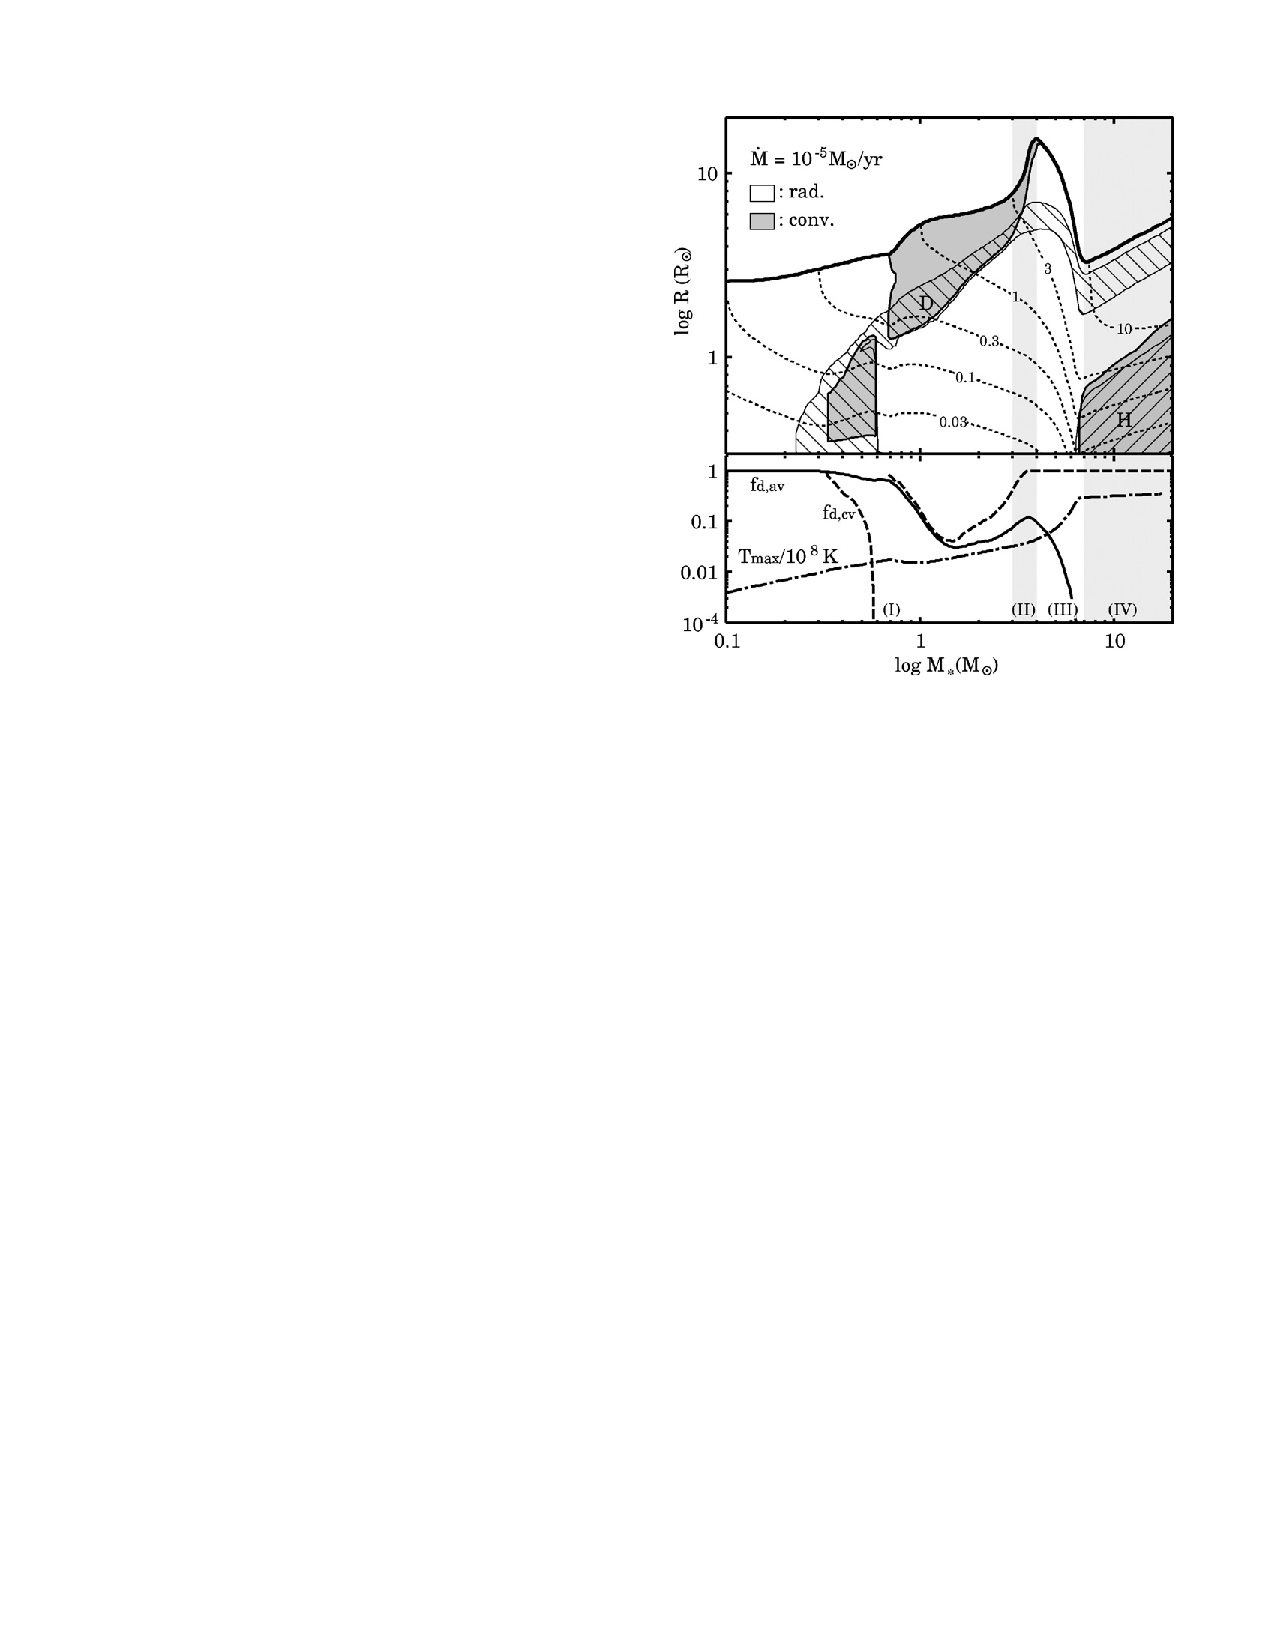
\includegraphics[width=\linewidth]{kippenhahn_hosokawa09}
\caption[Kippenhahn diagram for an accretion protostar]{
\label{fig:kippenhahn_hosokawa09}
Kippenhahn and composition diagrams for a protostar accreting at $10^{-5}$ $M_\odot$ yr$^{-1}$ \citep{hosokawa09a}. In the top panel, the thick curve shows the protostellar radius as a function of mass, and gray and white bands show convective and radiative regions, respectively. Hatched areas show regions of D and H burning, as indicated. Thin dotted lines show the radii containing $0.1$, $0.3$, $1$, $3$, and $10$ $M_\odot$, as indicated. Shaded regions show four evolutionary phases: (I) convection, (II) swelling, (III) KH-contraction, and (IV) the main sequence. In the lower panel, the solid line shows the mean deuterium fraction in the star, normalized to the starting value, while the dashed line shows the D fraction only considering the convective parts of the star. The dot-dashed line shows the maximum temperature.
}
\end{figure}

\subsection{Initial Contraction}

The initial phase of evolution is visible in Figure \ref{fig:kippenhahn_hosokawa09} as what takes place up to a mass of $\approx 0.2$ $M_\odot$ for the example shown. The first thing that happens during this phase is that the star reaches a radius that is a function solely of $M_*$ and $\dot{M}_*$. This occurs regardless of the initial radius with which we initiate the model, as long as we are using the hot accretion boundary condition. The physical reason for this behavior is easy to understand. The radius of the star is determined by the entropy profile $s(M_r)$. High entropy leads to high radius. Since the internal energy generated by the star is small compared to the accretion power when the stellar mass is low (i.e., $L_{\rm bb} \ll L_{\rm acc}$), once gas is incorporated into the star it does not lose significant energy by radiation. The only entropy it loses is due to the radiation that occurs at the shock on the star's surface. We could have guessed this result from the large value of $t_{\rm KH}$ compared to the accretion time -- in effect, this means that, once a fluid element reaches the stellar surface it will be buried and reach a nearly constant entropy quite quickly. Consequently, we can treat the material falling onto the star during this phase as having an entropy per unit mass that depends only on two factors: (1) the entropy it acquires by striking the stellar surface, and (2) how much it radiates before being buried.

The latter factor is just determined by the accretion rate. Higher accretion rates bury accreted material more quickly, leaving it with higher entropy and producing larger radii. The former depends on the velocity of the infalling material just before it strikes the stellar surface, and thus on $v_{\rm ff}\propto \sqrt{M_*/R_*}$. However, this second factor self-regulates. If at fixed $M_*$, $R_*$ is very large, then $v_{\rm ff}$ is small, and the incoming material gains very little entropy in the shock. Small entropy leads to a smaller radius. Conversely, if $R_*$ is very small, then $v_{\rm ff}$ and the post-shock entropy will be large, and this will produce rapid swelling of the protostar. This effect means that the radius rapidly converges to a value that depends only on $M_*$ and $\dot{M}_*$.

This self-regulation does not happen if the material is assumed to accretion cold. In this case, the radial evolution of the star is determined solely by the amount of entropy that is assumed to remain in the accretion flow when it joins onto the star. One common practice is to assume that the entropy of the accreting material is equal to the entropy of the gas already in the star, and, under this assumption, the choice of initial condition completely determines the subsequent evolution, since the choice of initial condition then determines the entropy content of the star thereafter.

Regardless of the boundary condition assumed, during this phase there is no nuclear burning in the star, as the interior is too cold for any such activity. Since there is no nuclear burning, and this phase generally lasts much less than the Kelvin-Helmholtz timescale on which radiation changes the star's structure, during this phase the entropy content of the star is nearly constant. This phase can therefore be referred to as the adiabatic stage in the star's evolution.


\subsection{Deuterium Ignition and Convection}

In Figure \ref{fig:kippenhahn_hosokawa09}, the next evolutionary phase begins at $\approx 0.25$ $M_\odot$, and continues to $\approx 0.7$ $M_\odot$. This stage is marked by two distinct but interrelated phenomena: the onset of nuclear burning and the onset of convection. The driving force behind both phenomena is that, as the protostar gains mass, its interior temperature rises. Recall the results of our calculation from Chapter \ref{ch:protostar_form}: for a polytrope, which is not an unreasonable description of the accreting protostar, the central temperature rises with mass to the $T_c\propto M^{(2\gamma-2)/(3\gamma-2)}$. Thus even at fixed entropy the central temperature must rise as the star gains mass.

Once $T_c$ reaches $\sim 10^6$ K, deuterium will ignite at the center of the protostar. This generally happens at a mass of hundredths to tenths of $M_\odot$, depending on the choice of accretion rate and boundary condition. This has two significant effects. The first is that deuterium acts as a thermostat for the star's center, much as hydrogen does in a main sequence star. Because the energy generation rate is so incredibly sensitive to $T$, any slight raise in the temperature causes it to jump enough to raise the pressure and adiabatically expand the star, reducing $T$. Thus, $T_c$ becomes fixed at $10^6$ K -- which is part of the reason we didn't need an expression for $\epsilon$ that would work at higher temperatures. The star adjusts its radius accordingly, which generally requires that the radius increase to keep $T_c$ nearly constant as the mass rises. Thus deuterium burning temporarily halts core contraction. Both effects are visible in Figure \ref{fig:kippenhahn_hosokawa09}. The halting of core contraction is apparent from the way the dotted lines showing constant mass enclosed bend upward at $\approx 0.3$ $M_\odot$, and the nearly constant core temperature is visible from the fact that, between $\approx 0.25$ $M_\odot$ and $3-4$ $M_\odot$, a factor of more than 10 in mass, the central temperature stays within a factor of 2 of $10^6$ K.

The second effect of deuterium burning that it causes a rapid rise in the entropy at the center of the star: looking at the heat equation (\ref{heat}), we can see that if $\epsilon$ is large, then $\partial s/\partial t$ will be as well. This has the effect of starting up convection in the star. Before deuterium burning the star is generally stable against convection. That is because the entropy profile is determined by infall, and since shells that fall onto the star later arrive at higher velocities (due to the rising $M_*$), they have higher entropy. Thus $s$ is an increasing function of $M_r$, which is the condition for convective stability. Deuterium burning reverses this, and convection follows, eventually turning much of the star convective. This also ensures the star a continuing supply of deuterium fuel, since convection will drag gas from the outer parts of the star down to the core, where they can be burned.

An important caveat here is that, although D burning encourages convection, it is not necessary for it. In the absence of D, or for very high accretion rates, the onset of convection is driven by the increasing luminosity of the stellar core as it undergoes KH contraction. This energy must be transported outwards, and as the star's mass rises and the luminosity goes up, eventually the energy that must be transported exceeds the ability of radiation to carry it. Convection results. For very high accretion rates, this effect drives the onset of convection even before the onset of D burning.

A third effect of the deuterium thermostat is that it forces the star to obey a nearly-linear mass-radius relation, and thus to obey a particular relationship between accretion rate and accretion luminosity. One can show that for a polytrope the central temperature and surface escape speed are related by
\begin{equation}
\psi = \frac{GM}{R} = \frac{1}{2}v_{\rm esc}^2 = T_n \frac{k_B T_c}{\mu m_{\rm H}},
\end{equation}
where $T_c$ is the core temperature, $T_n$ is a dimensionless constant of order unity that depends only on the polytropic index, and $\mu$ is the mean mass per particle in units of hydrogen masses. For $n=3/2$, expected for a fully convective star, $T_n = 1.86$. Plugging in this value of $T_n$, $\mu=0.61$ (the mean molecular weight for a fully ionized gas of H and He in the standard abundance ratio), and $T_c = 10^6$ K, one obtains $\psi = 2.5\times 10^{14}$ erg g$^{-1}$ as the energy yield from accretion.

\subsection{Deuterium Exhaustion and Formation of a Radiative Barrier}

The next evolutionary phase, which runs from $\approx 0.6 - 3$ $M_\odot$ in Figure \ref{fig:kippenhahn_hosokawa09}, is marked by the exhaustion of deuterium in the stellar core. Deuterium can only hold up the star for a finite amount of time. The reason is simply that there isn't that much of it. Each deuterium burned provides $5.5$ MeV of energy, comparable the $7$ MeV per hydrogen  provided by burning hydrogen, but there are only $2\times 10^{-5}$ D nuclei per H nuclei. Thus, at fixed luminosity the ``main sequence" lifetime for D burning is shorter than that for H burning by a factor of $2\times 10^{-5} \times 5.5/7 = 1.6\times 10^{-5}$.

We therefore see that, while a main sequence star can burn hydrogen for $\sim 10^{10}$ yr, a comparable pre-main sequence star of the same mass and luminosity burning deuterium can only do it for only a few times $10^5$ yr. To be more precise, the time required for a star to exhaust its deuterium is
\begin{equation}
t_{\rm D} = \frac{[\mbox{D}/\mbox{H}] \Delta E_{\rm D} M_*}{m_H L_*} = 1.5\times 10^6\mbox{ yr} \, M_{*,0} L_{*,0}^{-1}.
\end{equation}
Thus deuterium burning will briefly hold up a star's contraction, but cannot delay it for long. However, a brief note is in order here: while this delay is not long compared to the lifetime of a star, it is comparable to the formation time of the star. Recall that typical accretion rates are of order a few times $10^{-6}$ $\msun$ yr$^{-1}$, so a 1 $\msun$ star takes a few times $10^5$ yr to form. Thus stars may burn deuterium for most of the time they are accreting.

The exhaustion of deuterium does not mean the end of deuterium burning, since fresh deuterium that is brought to the star as it continues accreting will still burning. Instead, the exhaustion of core deuterium happens for a more subtle reason. As the deuterium supply begins to run out, the rate of energy generation in the core becomes insufficient to prevent it from undergoing further contraction, leading to rising temperatures. The rise in central temperature lowers the opacity, which is govern by a Kramers' law: $\kappa \propto \rho T^{-3.5}$. This in turn makes it easier for radiation to transport energy outward. Eventually this shuts off convection somewhere within the star, leading to formation of what is called a radiative barrier.

The formation of the barrier ends the transport of D to the stellar center. The tiny bit of D left in the core is quickly consumed, and, without D burning to drive an entropy gradient, convection shuts off through the entire core. This is the physics behind the nearly-simultaneous end of central D burning and central convection that occurs near $0.6$ $M_\odot$ in Figure \ref{fig:kippenhahn_hosokawa09}. After this transition, the core is able to resume contraction, and D continues to burn as fast as it accretes. However, it now does so in a shell around the core rather than in the core.

\subsection{Swelling}

The next evolutionary phase, which occurs from $\approx 3-4$ $M_\odot$ in Figure \ref{fig:kippenhahn_hosokawa09}, is swelling. This phase is marked by a marked increase in the star's radius over a relative short period of time. The physical mechanism driving this is the radiative barrier discussed above. The radiative barrier forms because increasing temperatures drive decreasing opacities, allowing more rapid transport of energy by radiation. The decreased opacity allows the center of the star to lose entropy rapidly, and the entropy to be transported to the outer parts of the star via radiation. The result is a wave of luminosity and entropy that propagates outward through the star.

\begin{marginfigure}
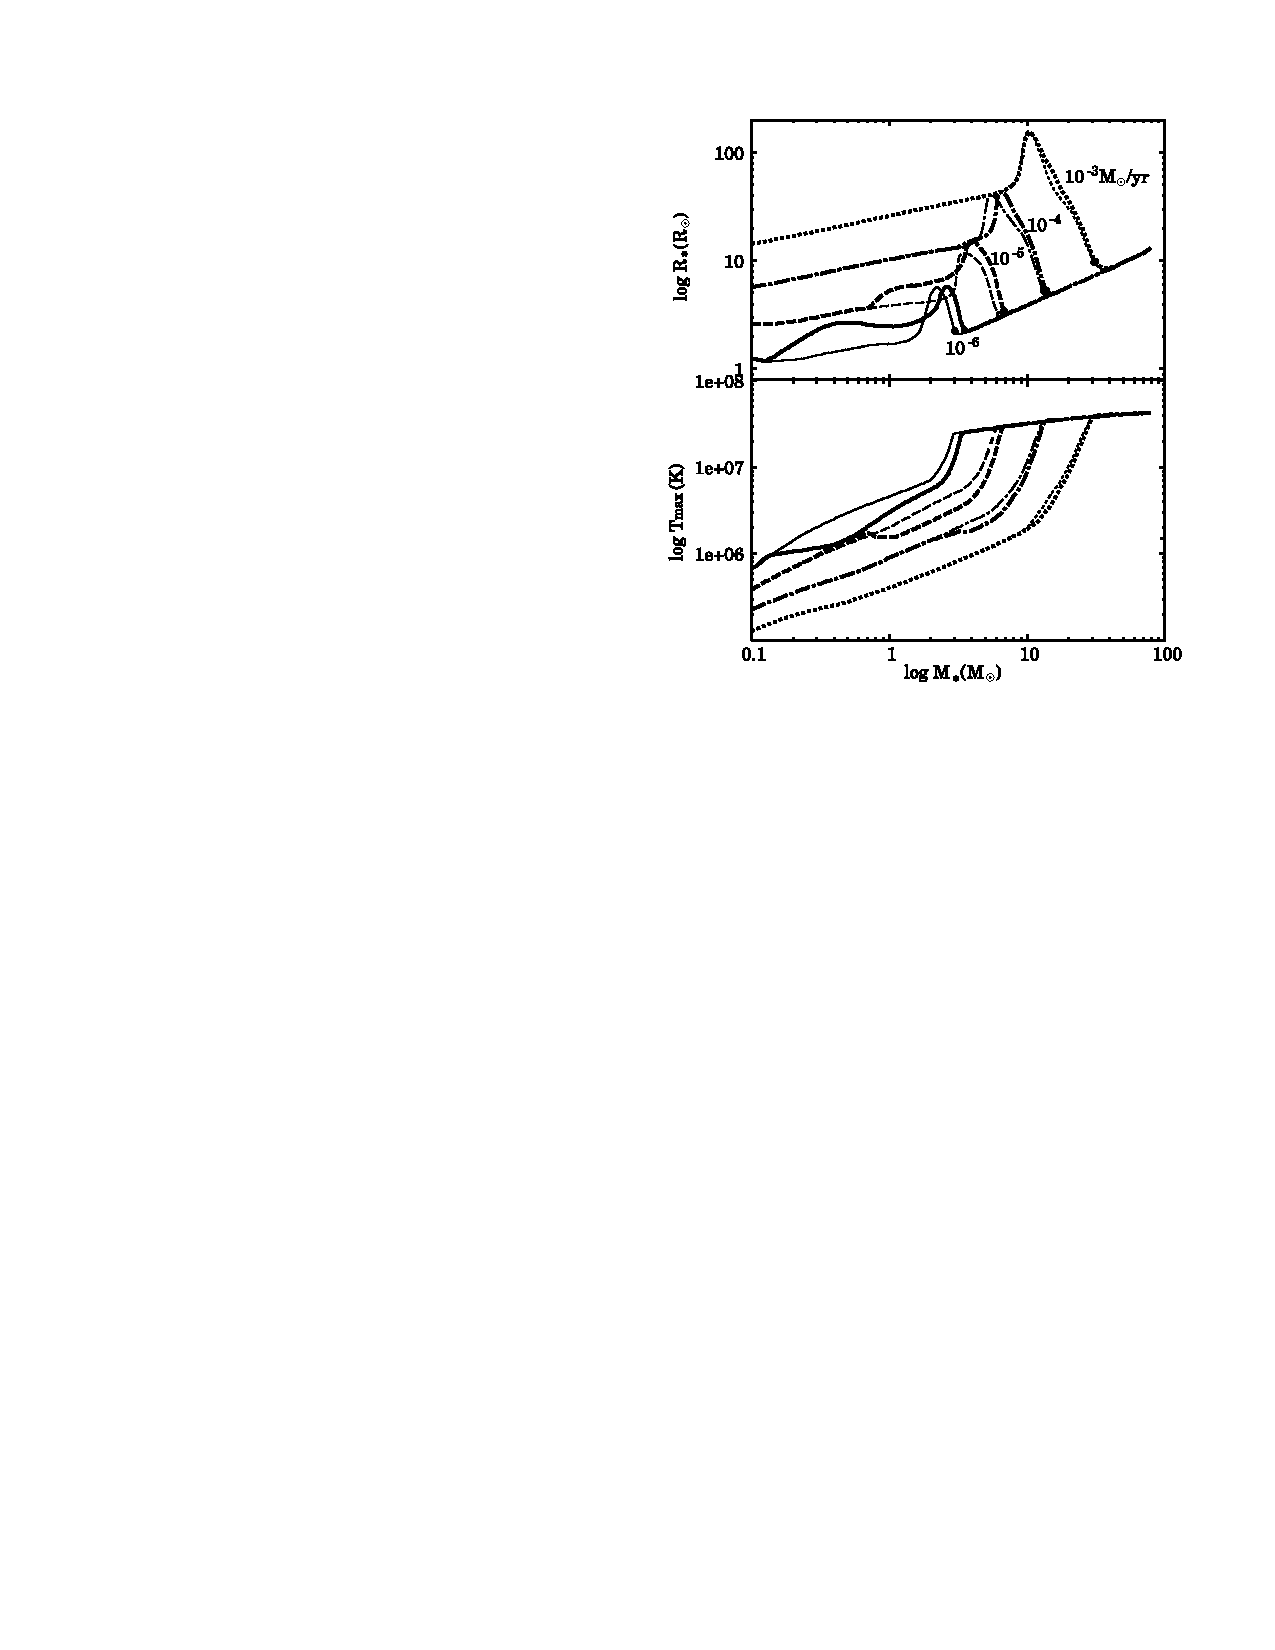
\includegraphics[width=\linewidth]{rt_hosokawa09}
\caption[Protostellar mass-radius relation for different accretion rates]{
\label{fig:rt_hosokawa09}
Radius versus mass (top panel) and maximum temperature versus mass (bottom panel) for protostars accreting at different rates. The accretion rate is indicated by the line style, as illustrated in the top panel. For each accretion rate there are two lines, one thick and one thin. The thick line is for the observed Milky Way deuterium abundance, while the thin line is the result assuming zero deuterium abundance.
}
\end{marginfigure}

Once the wave of luminosity and entropy gets near the stellar surface, which is not confined by the weight of overlying material, the surface undergoes a rapid expansion, leading to rapid swelling. The maximum radius, and the mass at which the swelling phase occurs, is a strong function of the accretion rate (Figure \ref{fig:rt_hosokawa09}). However, even at very low accretion rates, swelling does not occur until the mass exceeds $1$ $M_\odot$.

\subsection{Contraction to the Main Sequence}

The final stage of protostellar evolution is contraction to the main sequence. Once the entropy wave hits the surface, the star is able to begin losing energy and entropy fairly quickly, and it resumes contraction. This marks the final phase of protostellar evolution, visible above $\approx 4$ $M_\odot$ in Figure \ref{fig:kippenhahn_hosokawa09}. Contraction ends once the core temperature becomes hot enough to ignite hydrogen, landing the star at least on the main sequence.

\section{Observable Evolution of Protostars}


We have just discussed the interior behavior of an evolving protostar. While this is important, it is also critical to predict the observable properties of the star during this evolutionary sequence. In particular, we wish to understand the star's luminosity and effective temperature, which dictate its location in the HR diagram. The required values can simply be read off from the evolutionary models (Figure \ref{fig:pms_siess00}), giving rise to a track of luminosity versus effective temperature in the HR diagram. Our goal in the final section of this chapter is to understand those tracks.

\begin{marginfigure}
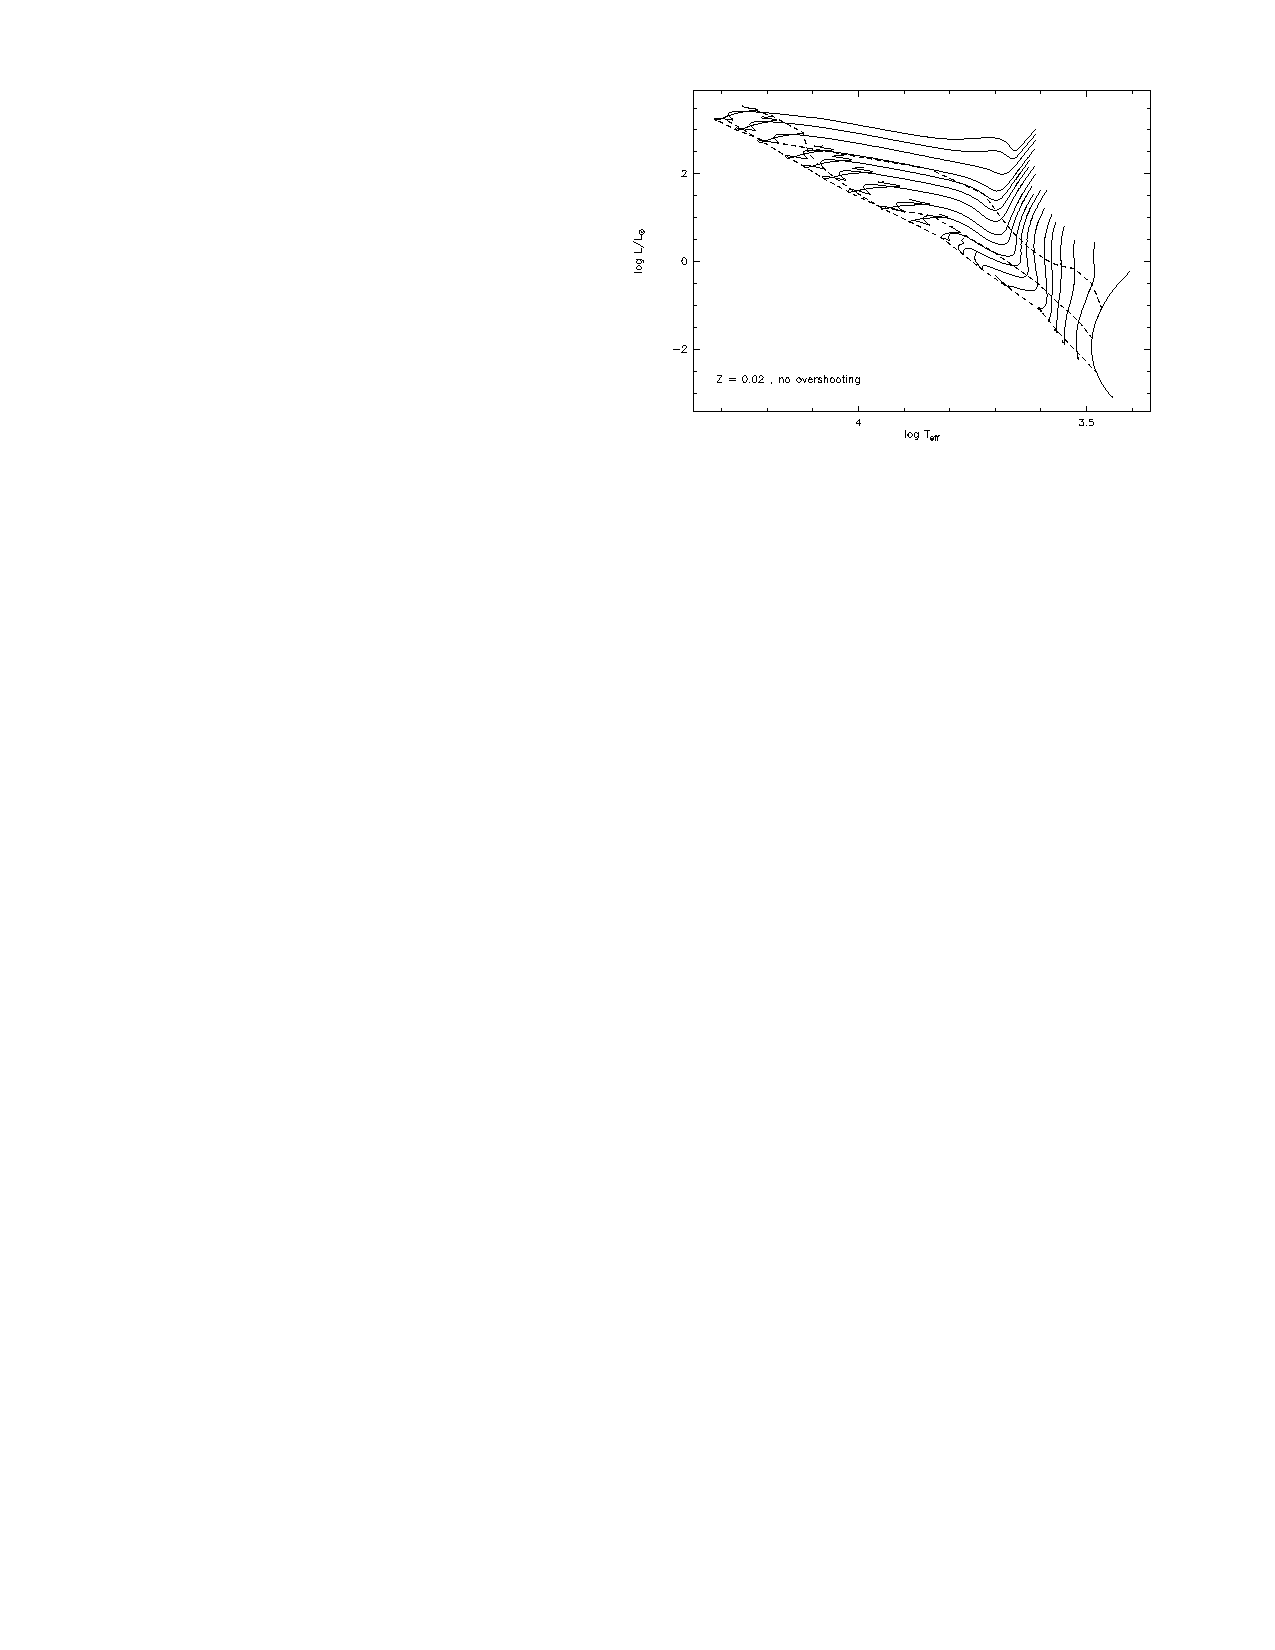
\includegraphics[width=\linewidth]{pms_siess00}
\caption[Pre-main sequence evolutionary tracks]{
\label{fig:pms_siess00}
Solid lines show tracks taken by stars of varying masses, from $0.1$ $M_\odot$ (rightmost line) to $7.0$ $M_\odot$ (leftmost line) in the theoretical HR diagram of luminosity versus effective temperature. Stars begin at the upper right of the tracks and evolve to the lower left; tracks end at the main sequence. Dashed lines represent isochrones corresponding to $10^6$, $10^7$, and $10^8$ yr, from top right to bottom left. Figure from \citet{siess00a}.
}
\end{marginfigure}

\subsection{The Birthline}

Before delving into the tracks themselves, we have to ask what is actually observable. As long as a star is accreting from its parent core, it will probably not be visible in the optical, due to the high opacity of the dusty gas in the core. Thus we are most concerned with stars' appearance in the HR diagram only after they have finished their main accretion phase. We refer to stars that are still accreting and thus not generally optically-observable as protostars, and those that are in this post-accretion phase as pre-main sequence stars. 

For stars below $\sim 1$ $M_\odot$, examining Figure \ref{fig:kippenhahn_hosokawa09}, we see that the transition from protostar to pre-main sequence star will occur some time after the onset of deuterium burning, either during the core or shell burning phases depending on the mass and accretion history. More massive stars will become visible only during KH contraction, or even after the onset of hydrogen burning. The lowest mass stars might be observable even before the start of deuterium burning. However, for the majority of the pre-main sequence stars that we can observe, they first become visible during the D burning phase.

\begin{marginfigure}
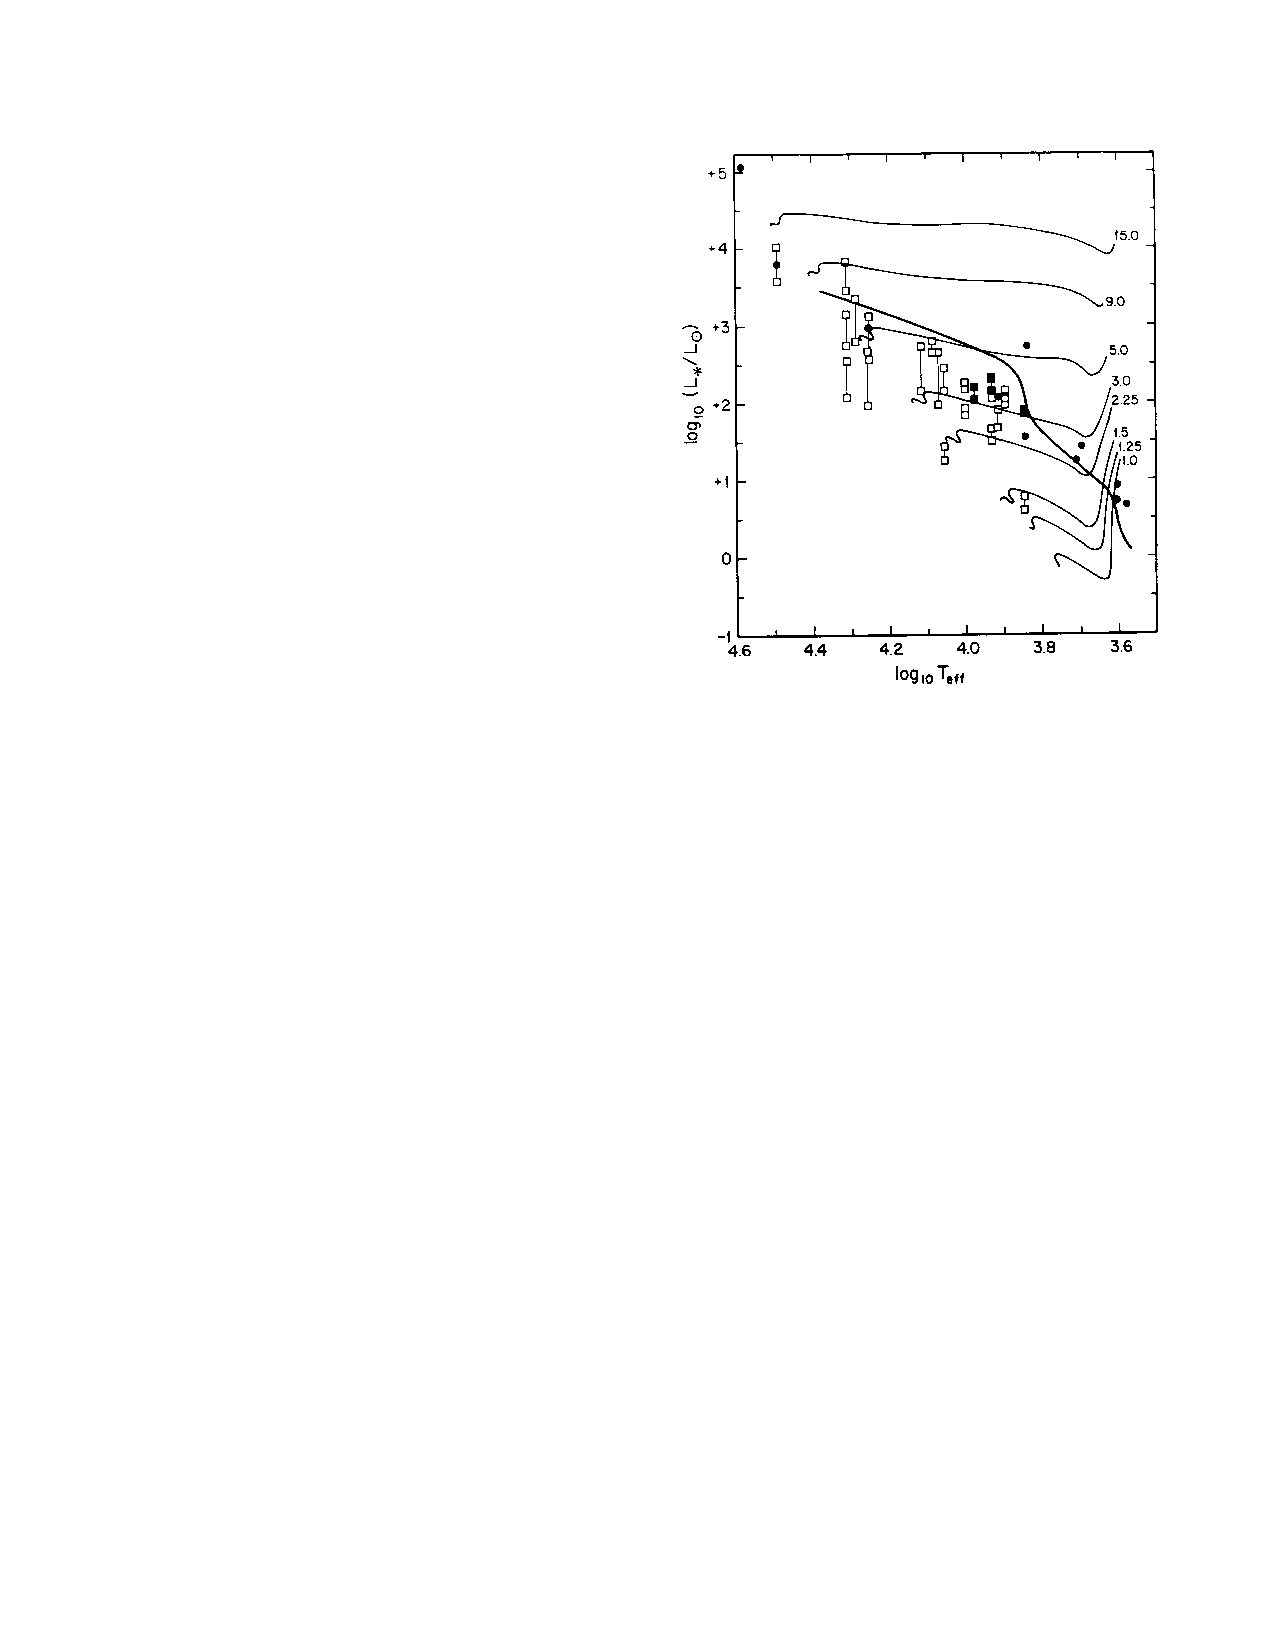
\includegraphics[width=\linewidth]{birthline_palla90}
\caption[The protostellar birthline]{
\label{fig:birthline_palla90}
Thin lines show tracks taken by stars of varying masses (indicated by the annotation, in $M_\odot$) in the theoretical HR diagram of luminosity versus effective temperature. Stars begin at the upper right of the tracks and evolve to the lower left; tracks end at the main sequence. The thick line crossing the tracks is the birthline, the point at which the stars stop accreting and become optically visible. Squares and circles represent the properties of observed young stars. Figure taken from \citet{palla90a}.
}
\end{marginfigure}

Since there is a strict mass-radius relation during core deuterium burning (with some variation due to varying accretion rates), there must be a corresponding relationship between $L$ and $T$, just like the main sequence. We call this line in the HR diagram, on which protostars first appear, the birthline; it was first described by \citet{palla90a} (Figure \ref{fig:birthline_palla90}). Since young stars are larger and more luminous that main sequence stars of the same mass, this line lies at higher $L$ and lower $T$ than the main sequence.

\subsection{The Hayashi Track}

Now that we understand what is observable, let us turn to the tracks themselves. The tracks shown in Figures \ref{fig:pms_siess00} and \ref{fig:birthline_palla90} show several distinct features. One is that, for low mass stars, the initial phases of evolution in the HR diagram are nearly vertically, i.e., at constant $T_{\rm eff}$. The vertical tracks for different masses are very close together. This vertical part of the evolution is called the Hayashi track, after its discoverer, who predicted it theoretically \citep{hayashi61a}. For low mass stars, the majority of the Hayashi track lies after the birthline, so it is directly observable.

The origin of the Hayashi track is in the physics of opacity in stellar atmospheres at low temperature. At temperatures below about $10^4$ K, hydrogen becomes neutral, and the only free electrons available come from metal atoms with lower ionization energies. Some of these electrons become bound with hydrogen atoms, forming H$^-$, and this ion is the dominant source of opacity.  Thus the opacity depends on the number of free electrons provided by metal atoms, which in turn depends extremely sensitively on the temperature.

If the temperature falls too low, the opacity will be so low that, even integrating through the rest of the star's mass, the optical depth to infinity will be $<2/3$. Since the photosphere must always be defined by a surface of optical depth unity, this effectively establishes a minimum surface temperature for the star required to maintain $\tau \approx 1$. This minimum temperature depends weakly on the star's mass and radius, but to good approximation it is simply $T_{\rm min} = T_{\rm H} = 3500$ K, where $T_{\rm H}$ is the Hayashi temperature. Low mass protostars, due to their large radii, wind up right against this limit, which is why they all contract along vertical tracks that are packed close together in $T_{\rm eff}$.

We can make this argument a bit more quantitative as follows. Let us approximate the stellar photosphere at radius $R$ as producing blackbody emission and obeying a simple ideal gas law equation of state. In this case we have
\begin{eqnarray}
\label{eq:bb}
\log L & = & 4 \log T_R - 2 \log R + \mbox{constant} \\
\label{eq:idealgas}
\log P_R & = & \log \rho_R + \log T_R + \mbox{constant},
\end{eqnarray}
where the subscript $R$ indicates that a quantity is to be evaluated at the stellar outer radius, and we are writing things in terms of logarithms rather than powerlaw scalings for future convenience. Now let us consider a star that is a polytrope, following $P\propto K_P \rho^{(n+1)/n}$. The polytropic constant$K_P$ is related to the stellar mass and radius by
\begin{equation}
K_P \propto M^{(n-1)/n}R^{(3-n)/n}.
\end{equation}
Thus we have
\begin{equation}
\log K_P = \left(\frac{n-1}{n}\right) \log M + \left(\frac{3-n}{n}\right)\log R + \mbox{constant},
\end{equation}
and the pressure scales with $M$ and $R$ as
\begin{equation}
\label{eq:polytrope}
\log P = \left(\frac{n-1}{n}\right) \log M + \left(\frac{3-n}{n}\right) \log R + \left(\frac{n+1}{n}\right) \log \rho + \mbox{constant}.
\end{equation}
Hydrostatic balance at the photosphere requires
\begin{equation}
\frac{dP}{dr} = \rho_R \frac{GM}{R^2} \qquad\Longrightarrow\qquad
P_R = \frac{GM}{R^2} \int_R^\infty \rho \, dr,
\end{equation}
where $P_R$ is the pressure at the photosphere and we are approximating the $GM/R^2$ is essentially constant through the photosphere. The photosphere is defined by the condition
\begin{equation}
\kappa \int_R^\infty \rho\,dr \approx 1,
\end{equation}
where we are also approximating $\kappa$ as constant, so putting this together we have
\begin{equation}
P_R \approx \frac{GM}{R^2\kappa} \qquad\Longrightarrow\qquad
\log P_R \approx \log M - 2 \log R - \log \kappa.
\end{equation}

To make further progress, we will assume that we can approximate the opacity as some powerlaw in density and temperature, $\kappa \propto \rho T^b$. For a Kramers opacity, for example, $a=1$ and $b=-3.5$. Substituting this into the equation for $P_R$, we have
\begin{equation}
\label{eq:opacity}
\log P_R = \log M - 2\log R - \log \rho_R - b\log T_R + \mbox{constant}.
\end{equation}

Equations (\ref{eq:bb}), (\ref{eq:idealgas}), (\ref{eq:polytrope}) and (\ref{eq:opacity}) constitute a system of four linear equations in the four unknowns $\log P_R$, $\log \rho_R$, $\log T_R$, and $\log L$. Solving this linear system yields the result
\begin{equation}
\log L = \left(\frac{9 - 2 n + b}{2-n}\right) \log T_R - \left(\frac{2n-1}{2-n}\right) \log M + \mbox{constant}.
\end{equation}
This equation describes the shape of a track in the HR diagram, because it relates $\log L$ to $\log T_R$, the photospheric temperature. To see what it implies, we can assume that young low mass stars will be fully convective thanks to D burning, so $n\approx 1.5$.

This leaves only $b$. As mentioned previously, the H$^{-}$ opacity has the property that it rises sharply with temperatures of a few thousand K, because at these temperatures collisional velocities are not high enough to dissociate H$^-$, but they are able to dissociate other atoms, which in turn produces free electrons that can yield H$^{-}$. The higher the temperature, the more free electrons available, and thus the higher the H$^{-}$ opacity. The net result is that, in this temperature range, $b$ takes on a fairly large value: $\sim 4-9$ depending on exactly where in the temperature range we are. Note that this is the opposite of the normal behavior for stellar opacities (e.g.\ Kramer's opacity), where the opacity falls with increasing temperature.

If we plug $b = 9$ and $n=1.5$ into the equation we have just derived, we find obtain
\begin{equation}
\log L = 30\log T_R - 4 \log M + \mbox{constant}.
\end{equation}
Using $b=4$ changes the 30 to a 20. Either way, we conclude that $\log L$ changes extremely steeply with $\log T_R$, which implies that the HR diagram track for stars with this low $T_{\rm eff}$ must be nearly vertical -- hence the Hayashi track. We also see that the location of the Hayashi tracks for stars of different masses will be slightly offset, because of the $4\log M$ term. This qualitatively explains what the numerical models produce.

\subsection{The Heyney Track}

Contraction at nearly constant $T_{\rm eff}$ continues until the star contracts enough to raise its surface temperature above $T_{\rm H}$. This increase in temperature also causes the star to transition from convective to radiative, since the opacity drops with temperature at high temperatures, and a lower opacity lets radiation rather than convection carry the energy outward.

In the HR diagram, the contraction and increase in $T_{\rm eff}$ produces a vaguely horizontal evolutionary track. This is called the Heyney track. The star continues to contract until its center becomes warm enough to allow H burning to begin.
At that point it may contract a small additional amount, but the star is essentially on the main sequence. The total time required depends on the stellar mass, but it ranges from several hundred Myr for $0.1$ $\msun$ stars to essentially zero time for very massive stars, which reach the main sequence while still accreting.


